% !TEX root = ../TensorOT.tex



%%%%%%%%%%%%%%%%%%%%%%%%%%%%%%%%%%%%%%%%%%%%%%%%%%%%%%%%%
\section{Quantum Barycenters}
\label{sec-q-bary}

Following Agueh and Carlier~\shortcite{agueh-2011} (see also~\cite{benamou-2015,solomon-2015} for numerical methods using entropic regularization), we now propose a generalization of the OT problem~\eqref{eq-Kantorovich}, where, instead of coupling only two input measures, one tries to couple an arbitrary set of inputs, and compute their Fr\'echet means. 

\newcommand{\weight}{w}

%%%%
\subsection{Barycenter Optimization Problem}

Given some input measures $(\mu^\ell)_\ell$, the quantum barycenter problem reads
\eql{\label{eq-defn-barycenters}
	\umin{\nu} \sum_\ell \weight_\ell W_\epsilon(\mu^\ell,\nu), 
}
where $(\weight_\ell)_\ell$ is a set of positive weights normalized so that $\sum_\ell \weight_\ell=1$. In the following, for simplicity, we set
\eq{
	\rho_1 = \rho 
	\qandq
	\rho_2 = +\infty
}
in the definition~\eqref{eq-Kantorovich} of $W_\epsilon$. Note that the choice $\rho_2=+\infty$ corresponds to imposing the exact hard marginal constraint $\gamma^\top \ones_J=\nu$. 

\begin{rem}[Barycenters between single Dirac masses]
	If all the input measures are concentrated on single Diracs $\mu^\ell=P_\ell \de_{x_\ell}$, then the single Dirac barycenter (unregularized, i.e., $\epsilon=0$) for a cost $d_X(x,y)^\al \Id_{d \times d}$ is $P \de_x^\star$ where $x^\star \in X$ is the usual barycenter for the distance $d_X$, solving 
	\eq{
		x^\star \in \argmin_{x} 
			\Ee(x) = \sum_\ell \weight_\ell d_X^\al(x_\ell,x) 
	}
	and the barycentric matrix is
	\eql{\label{eq-barycentric-matrix}
		P = e^{-\frac{\Ee(x^\star)}{\rho}} \exp\Big(\sum_{\ell} \weight_\ell \log(P_\ell)\Big).
	}
	Figure~\ref{fig:interp} illustrates the effect of a pointwise interpolation (i.e. at the same location $x_\ell$ for all $\ell$) between tensors.
\end{rem}


%%%%%%%%%%%%%%%%%%%%%%%%%%%%%%%%
\begin{figure}\centering
\fbox{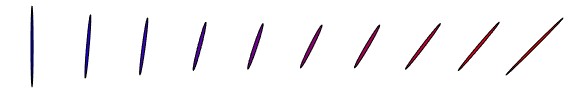
\includegraphics[width=.46\linewidth]{pointwise-interp/interp-rot_small-hard.png}}
\fbox{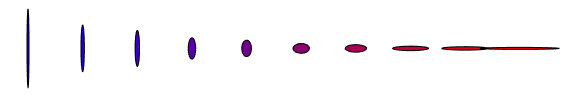
\includegraphics[width=.46\linewidth]{pointwise-interp/interp-ortho-hard.png}}
\caption{Two examples of pointwise (without transportation) interpolations, using formula~\eqref{eq-barycentric-matrix}. Here $P_1$ and $P_2$ are represented using the blue/red ellipses on the left/right, and weights are $(w_1,w_2)=(1-t,t)$ for $t \in [0,1]$ from left to right.} \label{fig:interp}
\end{figure}
%%%%%%%%%%%%%%%%%%%%%%%%%%%%%%%%




%%
\newcommand{\BaryImg}[2]{{\includegraphics[width=.095\linewidth,trim=18 160 18 160,clip]{2d-bary/barycenter-#1-#2}}}
\newcommand{\BaryImgLine}[1]{%%%
\BaryImg{#1}{1}&\BaryImg{#1}{2}&\BaryImg{#1}{3}&\BaryImg{#1}{4}&\BaryImg{#1}{5} %%%
}
%%
\newcommand{\BarySurf}[2]{{\includegraphics[width=.095\linewidth,trim=25 10 25 10,clip]{mesh-bary/barycenter-#1-#2}}}
\newcommand{\BarySurfLine}[1]{%%%
\BarySurf{#1}{1}&\BarySurf{#1}{2}&\BarySurf{#1}{3}&\BarySurf{#1}{4}&\BarySurf{#1}{5} %%%
}
%%

%%%%%%%%%%%%%%%%%%%%%%%%%%%%%%%%
%%
\begin{figure*}\centering
%%%%%
\begin{tabular}{@{}c@{}c@{}c@{}c@{}c@{}}
\BaryImgLine{1}\\
\BaryImgLine{2}\\
\BaryImgLine{3}\\
\BaryImgLine{4}\\
\BaryImgLine{5}
\end{tabular}
%%%%%
\hspace{5mm}
%%%%%
\begin{tabular}{@{}c@{}c@{}c@{}c@{}c@{}}
\BarySurfLine{1}\\
\BarySurfLine{2}\\
\BarySurfLine{3}\\
\BarySurfLine{4}\\
\BarySurfLine{5}
\end{tabular}
%%%%%
\caption{$5 \times 5$ barycenters of four input measures (displayed in the four corners). The weighs $w \in \RR^4$ corresponds to bilinear interpolation weights~\eqref{eq-bilinear} inside the square.
} \label{fig:barycenters}
\end{figure*}
%%%%%%%%%%%%%%%%%%%%%%%%%%%%%%%%


Problem~\eqref{eq-defn-barycenters} is convex, and similarly to~\eqref{eq-dual-pb}, it can be rewritten in dual form.

\begin{prop}
The optimal $\nu$ solving~\eqref{eq-defn-barycenters} is the solution of
\begin{multline}\label{eq-dual-bary}		
		\umax{(u^\ell,v^\ell)} \umin{\nu}
				- 
				\sum_\ell w_\ell 
					\tr\Big[
						\rho \sum_i e^{u_i^\ell+\log(\mu_i^\ell)} \\
					+    \sum_j \nu_j v_j^\ell
					+    \epsilon \sum_{i,j}  e^{ \Kern(u^\ell,v^\ell)_{i,j} }
			 \Big], 
\end{multline}	
\justin{Why is this equation broken up?} where here we define $\Kern$ as
\eql{\label{eq-def-k-bary}
	\Kern(u,v)_{i,j} \eqdef -\frac{c_{i,j} + \rho u_i +  v_j}{\epsilon}.
}
\end{prop}



\begin{algorithm}[t]
\fbox{\hspace{-.1in}\parbox{\columnwidth}{%
\begin{algorithmic}
\Function{Quantum-Barycenter}{$(\mu_\ell)_{\ell=1}^L,c,\epsilon,\rho$}
	% \LineComment{Computes minimizer $\ga$ of~\eqref{eq-Kantorovich-regul}}
	\algspace
	\State Choose $\tau_1 \in ]0,\tfrac{2 \epsilon}{\epsilon+\rho}[$, 
		$\tau_2 \in ]0,2[$.
	\Let{$\foralls (i,j) \in I \times J, \quad (u_i,v_j)$}{$(0_{d \times d}, 0_{d \times d})$}
	\For{$s=1,2,3,\ldots$.}
		%%%%
		\For{$\ell=1,\ldots,L$}
			\Let{$K^\ell$}{$\Kern(u^\ell,v^\ell)$, }
			\State $\foralls i \in I, \quad u_i^\ell \RelaxAssign{\tau_1} \LSE_j(K_{i,j}^\ell)-\log(\mu_i^\ell)$, 
			\Let{$K^\ell$}{$\Kern(u^\ell,v^\ell)$.}
		\EndFor
		%%%%
		\State $\foralls j \in J, \quad \log(\nu_j) \leftarrow 
			\sum_\ell w_\ell ( \LSE_i(K_{i,j}^\ell) + v^\ell_j/\epsilon ).$
		%%%%
		\For{$\ell=1,\ldots,L$}
			\State $\foralls j \in J, \quad v_j^\ell \RelaxAssign{\tau_2} \epsilon \LSE_i(K_{i,j}^\ell) + v^\ell_j - \epsilon \log(\nu_j).$	
		\EndFor		
	\EndFor
%	\algspace
	\State\Return{$\nu$}
\EndFunction
  \end{algorithmic}
}}
\caption{Quantum-Barycenter iterations to compute the optimal barycenter measure $\nu$ solving~\eqref{eq-defn-barycenters}. The operator $\Kern$ is defined in~\eqref{eq-def-k-bary}. \label{alg:barycenter}}
\end{algorithm}


%%%%
\subsection{Quantum Barycenter Sinkhorn}

Similarly to Proposition~\ref{prop-fixed-points}, the dual solutions of~\eqref{eq-dual-bary} satisfy a set of coupled fixed point equations:

\begin{prop}
Optimal $(u^\ell,v^\ell)_\ell$ for~\eqref{eq-dual-bary} satisfy 
\begin{align}
	\foralls (i,\ell), \quad \LSE_j(\Kern(u^\ell,v^\ell)_{i,j})-\log(\mu_i^\ell), \label{eq-fixed-point-u-bary} 
		&= u_i^\ell \\
	\foralls (j,\ell), \quad \LSE_i(\Kern(u^\ell,v^\ell)_{i,j}) \label{eq-fixed-point-v-bary}
		&= \log(\nu_j)\\ 
		 \textstyle \sum_\ell \weight_\ell v^\ell &= 0. \label{eq-fixed-point-nu-bary}
\end{align}
\end{prop}
\begin{proof}
The proof of~\eqref{eq-fixed-point-u-bary} and~\eqref{eq-fixed-point-v-bary} is the same as the one of Proposition~\ref{prop-fixed-points}.
%%
Minimization of~\eqref{eq-dual-bary} on $\nu$ leads to~\eqref{eq-fixed-point-nu-bary}. 
\end{proof}

The extension of the quantum Sinkhorn algorithm to solve the barycenter problem~\eqref{alg:barycenter} is detailed in Algorithm~\ref{alg:barycenter}. It alternates between the updates of $u$, $\nu$ and $v$, using the relaxed version of the fixed point equations~\eqref{eq-fixed-point-u-bary}, \eqref{eq-fixed-point-v-bary} and~\eqref{eq-fixed-point-nu-bary}. The notation $\RelaxAssign{\tau}$ refers to a relaxed assignment as defined in~\eqref{eq-dfn-relaxed-assign}. 

\begin{rem}[Choice of $\tau$]
Remark~\ref{rem-choice-tau} also applies for this Sinkhorn-like scheme, and setting $(\tau_1,\tau_2)=(\tfrac{\epsilon}{\rho+\epsilon},1)$ leads, in the scalar case $d=1$, to the algorithm in~\cite{2016-chizat-sinkhorn}. We found experimentally that this choice leads to contracting (and hence linearly converging) iterations, and that higher values of $\tau$ usually accelerate the convergence rate. 
\end{rem}

\begin{rem}[Scalar and isotropic cases]
Note that in the scalar case $d=1$ and for isotropic input tensors (multiples of the identity), one retrieves the provably convergent unbalanced barycenter algorithm in~\cite{2016-chizat-sinkhorn}.
\end{rem}




%%%%%%%%%%%%%%%%%%%%%%%%%%%%%%%%%%%%%%%%%%%%%%%%
\subsection{Numerical Illustrations}

Figure~\ref{fig:barycenters} shows examples of barycenters $\nu$ solving~\eqref{eq-defn-barycenters} between four input measures $(\mu^\ell)_{\ell=1}^4$. The horizontal/vertical axes of the figures are indexed by $(t_1,t_2) \in [0,1]^2$ (on a $5 \times 5$ grids) and parameterize the weights $(w_\ell)_{\ell=1}^4$ appearing in~\eqref{eq-defn-barycenters} as
\eql{\label{eq-bilinear}
	(w_1,w_2,w_3,w_4) \eqdef ( (1-t_1)(1-t_2), (1-t_1)t_2, t_1(1-t_2), t_1,t_2 ). 
}
The left part of Figure~\ref{fig:barycenters} corresponds to measures on $X=Y=[0,1]^2$ with $d=2$ and ground cost $c_{i,j}=\norm{x_i-x_j}^2\Id_{2 \times 2}$.
%
The right part of Figure~\ref{fig:barycenters} corresponds to measures on $X=Y$ being a surface mesh with $d=2$ (the tensors are defined on the tangent planes) and a ground cost is $c_{i,j}=d_X(x_i,x_j)^2\Id_{2 \times 2}$ where $d_X$ is the geodesic distance on the mesh.




